\usetikzlibrary{shadows,arrows}
\usetikzlibrary{decorations.markings}

% Define the layers to draw the diagram
\pgfdeclarelayer{background}
\pgfdeclarelayer{foreground}
\pgfsetlayers{background,main,foreground}

% Define block styles  
\tikzstyle{rectangle}=[draw, fill=blue!20, text width=6.0em, text centered,
  minimum height=1.5em,drop shadow]
\tikzstyle{practica} = [rectangle, text width=8em, minimum width=10em,
  minimum height=3em, rounded corners, drop shadow]

\tikzstyle{long} = [rectangle, text width=8em, minimum width=26em,
  minimum height=3em, rounded corners, drop shadow]

\tikzstyle{yoloswag}=[draw, fill=red!20, text width=6.0em, text centered,
  minimum height=1.5em,drop shadow]
\tikzstyle{redBox} = [yoloswag, text width=8em, minimum width=10em,
  minimum height=3em, rounded corners, drop shadow]

\tikzstyle{texto} = [above, text width=6em, text centered]

\tikzset{
    big arrow/.style={
        decoration={markings,mark=at position 1 with {\arrow[scale=2,#1]{>}}},
        postaction={decorate},
        shorten >=0.4pt}}
\tikzstyle{line} = [draw, thick, color=black!50, big arrow]
% Define distances for bordering

\newcommand{\practica}[2]{node (p#1) [practica] {#2}}
\newcommand{\redBox}[2]{node (p#1) [redBox] {#2}}
\newcommand{\longhorse}[2]{node (p#1) [long] {#2}}
\newcommand{\implemented}[2]{node (p#1) [interface] {#2}}
 
% Draw background
\newcommand{\backgroundDB}[5]{%
  \begin{pgfonlayer}{background}
    % Left-top corner of the background rectangle
    \path (#1.west |- #2.north)+(-0.5,0.5) node (a1) {};
    % Right-bottom corner of the background rectanle
    \path (#3.east |- #4.south)+(+0.5,-0.5) node (a2) {};
    % Draw the background
    \path[fill=green!20,rounded corners, draw=black!50, dashed]
      (a1) rectangle (a2);
    \path (a1.east |- a1.south)+(0.8,-0.3) node (u1)[texto]
      {\scriptsize\textit{#5}};
  \end{pgfonlayer}}
\newcommand{\background}[5]{%
  \begin{pgfonlayer}{background}
    % Left-top corner of the background rectangle
    \path (#1.west |- #2.north)+(-0.9,1.1) node (a1) {};
    % Right-bottom corner of the background rectanle
    \path (#3.east |- #4.south)+(+1.0,-1.00) node (a2) {};
    % Draw the background
    \path[fill=yellow!20,rounded corners, draw=black!50, dashed]
      (a1) rectangle (a2);
    \path (a1.east |- a1.south)+(1.0,-0.5) node (u1)[texto]
    {\scriptsize\textit{#5}};
  \end{pgfonlayer}} 
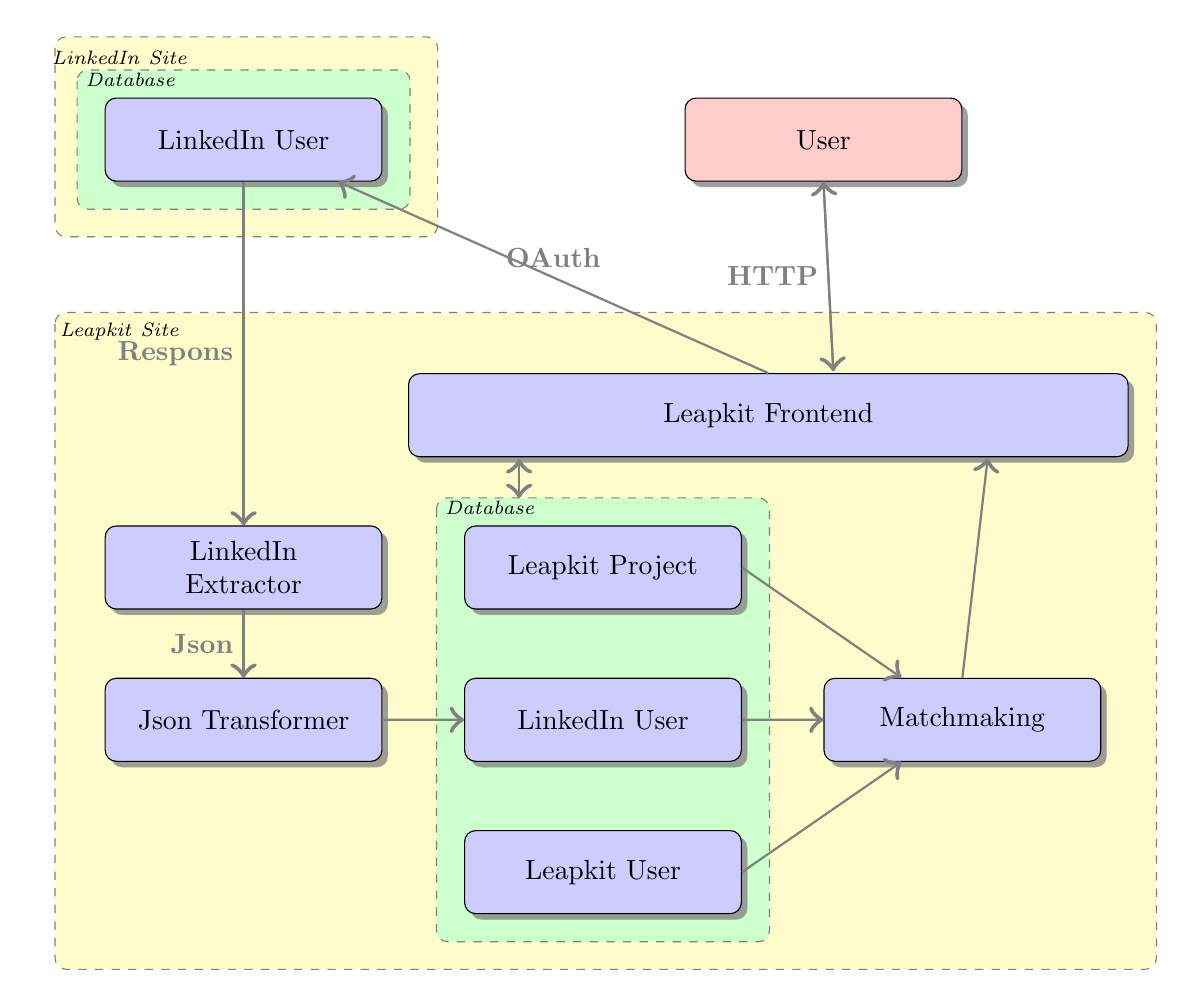
\begin{tikzpicture}[scale = 0.7]
% Draw diagram elements
\path                          \practica{1}{LinkedIn User};

\path (p1.south) +( 0.0,-7.0) \practica{2}{LinkedIn Extractor};
\path (p2.south) +( 0.0,-2.0) \practica{3}{Json Transformer};

\path (p2.east)+(4.0,0.0) \practica{7}{Leapkit Project};
\path (p7.south)+(0.0,-2.0) \practica{6}{LinkedIn User};
\path (p6.south)+(0.0,-2.0) \practica{8}{Leapkit User};
 
\path (p6.east)+(4.0,0.0) \practica{9}{Matchmaking};
\path (p7.north)+(3.0,2.0) \longhorse{10}{Leapkit Frontend};

\path (p1.east)+(8.0,0.0) \redBox{11}{User};

% Draw arrows between elements
\path [line] (p10.north) -- node [above] {\textbf{OAuth}} (p1);
\path [line] (p1.south) -- node [left] {\textbf{Respons}} (p2);

\path [line] (p2.south) -- node [left] {\textbf{Json}} (p3);

\path [line] (p3.east) -- (p6);
\path [line] (p6.east) -- (p9);
\path [line] (p7.east) -- (p9);
\path [line] (p8.east) -- (p9);
\path [line] (p9.north) -- (13.5,-5.78);
\path [line] (p11.south) -- (10.7, -4.2);
\path [line] (10.7, -4.2) -- node [left] {\textbf{HTTP}} (p11.south);

\background{p1}{p1}{p1}{p1}{LinkedIn Site}
\backgroundDB{p1}{p1}{p1}{p1}{Database}

\background{p2}{p10}{p9}{p8}{Leapkit Site}
\path [line] (5,-6.5) -- (5,-5.8);
\path [line] (5,-5.8) -- (5,-6.5);
\backgroundDB{p7}{p7}{p8}{p8}{Database}
\end{tikzpicture}
